\documentclass[a4paper,12pt]{article}

\usepackage[pdftex]{graphicx}
\usepackage[pdftex,breaklinks=true,colorlinks=true,linkcolor=black,filecolor=blue,urlcolor=blue]{hyperref}
\usepackage{color}
\usepackage[paper=a4paper,hmargin=2cm,vmargin=3cm]{geometry}
\usepackage{lscape}
\usepackage{amsmath}

% Paragraph style
\setlength\parindent{0in}
\setlength\parskip{0.1in}

% URL style
\def\UrlFont{\small\tt}

%opening
\title{COMP6026 Assignment 2 \\
An Evolutionary Approach to Tetris}
\author{David Sansome $<$ds505$>$}

\begin{document}
\bibliographystyle{plain}

\maketitle

\begin{abstract}

This report describes the design, implementation and results of an evolutionary
algorithm that plays the popular game of Tetris \cite{AboutTetris}.
Tetris is a falling-block game where the aim is to survive as long as possible
by dropping blocks (\emph{Tetraminos}) into a fixed-size board.
A row is cleared from the board if it is completely filled, and the game ends
when there is no more room in the board for new blocks.
The challenge therefore is to place blocks in such a way as to minimize holes
in the board and to clear as many rows as possible.

The algorithm used is as described by Mandl et.\ al \cite{Mandl2005}.
At each step of the game the computer evaluates all possible subsequent boards
and chooses the best move based on a rating function.
This function is a weighted sum of various board attributes, such as the height
of filled cells and the number of holes in the board.
The algorithm evolves the weights used in this function and finds sets of
weights that lead to longer games of Tetris.

Our implementation uses fitness proportional selection and uniform crossover.

\end{abstract}

\tableofcontents

\section{Methods}

\subsection{Representation of Individuals}

Each individual in the population is essentially a different \emph{board
rating function}.
The individual uses its board rating function at each step of the game to
decide where to place each block, choosing the move that will lead to the board
with the best score.
Individuals with better board rating functions will therefore make better moves
and last longer than the other individuals.

The board rating function is a weighted sum of the following six criteria:

\begin{enumerate}
  \item \emph{Pile Height}: The total height of the Tetris board, measured from
      the bottom of the board to the highest occupied cell.
  \item \emph{Holes}: The number of unoccupied cells that have at least one
      occupied cell above them.
  \item \emph{Connected Holes}: Same as \emph{Holes}, except vertically
      connected unoccupied cells only count as one connected hole.
  \item \emph{Removed Lines}: The number of lines that were cleared in the last
      step to get to the current board.
  \item \emph{Altitide Difference}: The difference between the highest occupied
      cell and the lowest free cell that are directly reachable from the top.
  \item \emph{Maximum Well Depth}: The depth of the deepest well on the board.
      A well is a vertical group of unoccupied cells with a width of one,
      reachable from the top and with other filled cells on both sides.
\end{enumerate}

\begin{figure}[hb]
  \centering
  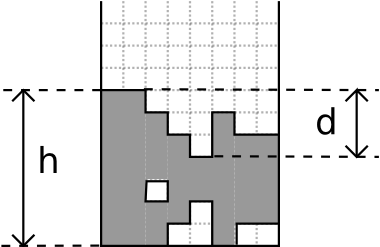
\includegraphics[width=5cm]{boards1.png}
  \caption{A Tetris board showing two of the rating criteria.  $h$ is
      the \emph{Pile Height}, or distance from the bottom of the board to
      the highest occupied cell.  $d$ is the \emph{Altitiude Difference}, or
      distance from the highest occupied cell to the lowest occupied cell
      reachable from the top of the board.}
  \label{BoardRating}
\end{figure}

The algorithm described by Mandl et.\ al uses these six criteria as well as
an additional six found in Colin Fahey's ``Standard Tetris Application''
\cite{TetrisAI}, however only these original six were used in our
implementation.

The six criteria ($r_i$) are combined to create the overall linear rating
function $R_l(b)$:

\begin{equation}
  R_l(b) = \sum^6_{i=1} w_ir_i(b)
\end{equation}

Mandl describes two other possible rating functions which give a closer
approximation to the way a human player evaluates the Tetris board.
There is no big difference between pile heights of 2 and 4, but a difference
between heights of 15 and 17 has a much more drastic influence on the game.
The exponential rating function $R_e(b)$ is useful because it treats these two
scenarios differently.
The third rating function $R_d(b)$ uses the idea that the optimum value for a
certain criteria might not be zero.

\begin{equation}
  R_e(b) = \sum^6_{i=1} w_ir_i(b)^{e_i}
\end{equation}

\begin{equation}
  R_d(b) = \sum^6_{i=1} w_i \lvert r_i(b) - d_i \rvert ^{e_i}
\end{equation}

Although Mandl evaluates all three rating functions, only the simple linear
rating function $R_l(b)$ is used in this implementation.

Each individual therefore consists of one \emph{weights} chromosome
($w_1, \ldots, w_6$) with each of $w_i$ being an integer number.

\subsection{Fitness Evaluation}

The fitness of each individual genotype is measured on the phenotype.
In other words, an instance of the board rating function is created and it is
allowed to play a game of Tetris.
The fitness of the rating function is taken to be the number of blocks it
manages to place before the game ends.

Other possible methods of determining fitness include counting cleared lines
and counting ``points'' for different kinds of actions (for example, scoring
bonus points from clearing more than one line with a single block).

There is a strong random component to the success of an individual in a game of
Tetris (due to the randomness of the upcoming Tetraminos), so each individual
is allowed to play a number of games (usually around 12), and the mean number
of blocks placed each time is taken as its fitness.

\subsection{Generational}
\subsection{Selection}
\subsection{Crossover and Mutation}
\subsection{Implementation Details}

\section{Results}

\section{Further Work}

\bibliography{../COMP6026}

\end{document}
